\subsection{Extration of Connected Components}
 
Figur~\ref{fig:connected-component} viser ligningen for denne ''extraction''. Vi finder et punkt i en component (typisk efter thresholding) og bruger dialation på denne, så længe vi stadig er indeholdt i komponenten og ikke går udenfor.

\begin{figure}[H]
	\centering
	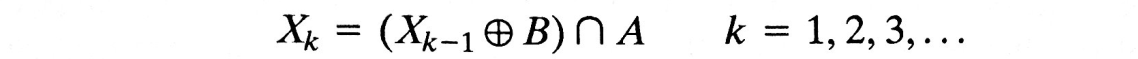
\includegraphics[width=0.7\linewidth]{figs/spm10/connected-component}
	\caption{Ligning for extraction of connected components.}
	\label{fig:connected-component}
\end{figure}

Figur~\ref{fig:connected-component-example} viser et eksempel på denne algoritme.

\begin{figure}[H]
	\centering
	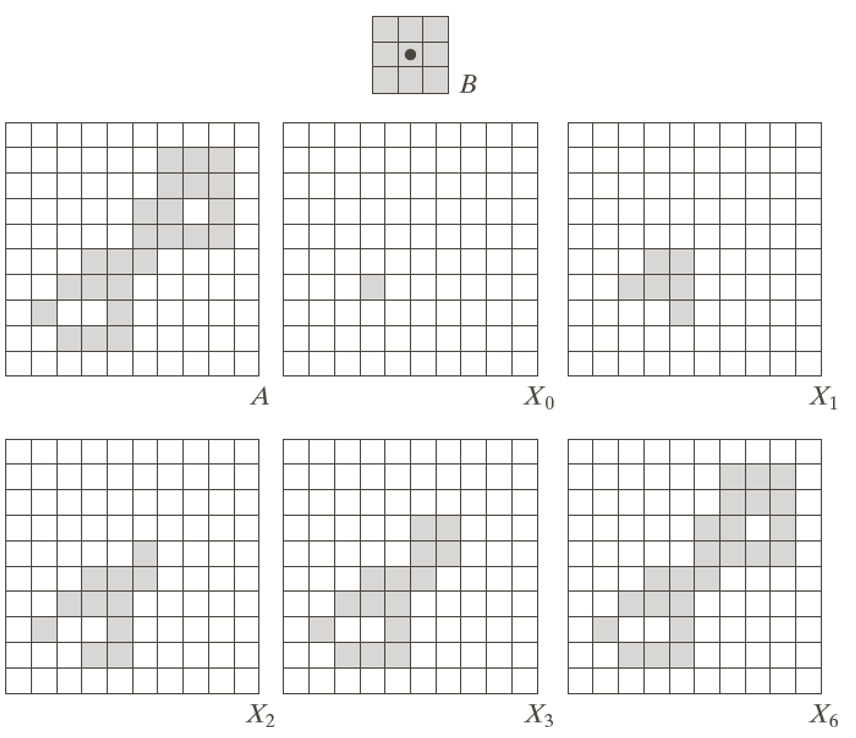
\includegraphics[width=0.9\linewidth]{figs/spm10/connected-component-example}
	\caption{Eksempel på componenet extraction.}
	\label{fig:connected-component-example}
\end{figure}
